\subsection{Hjertet}

\subsection{Elektrokardiogram}

\begin{figure}[H]
\centering
  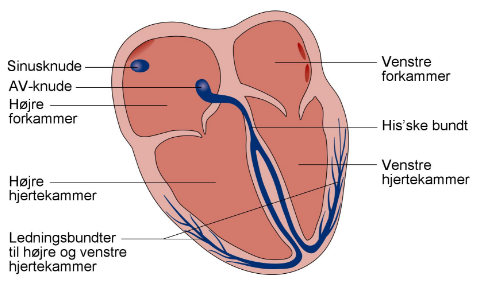
\includegraphics[width=0.6\textwidth]{Billeder/hjerte.png}
   \caption{Hjertets anatomi fra sundhed.dk} 
   \label{fig:hjerte}
\end{figure}

Hvert hjerteslag udløses af en lille specialiseret gruppe af celler, som kaldes sinusknuden og er hjertets naturlige pacemaker. Sinusknuden har evnen til at udløse elektriske signaler - også kaldet impulser - som er begyndelsen på et hjerteslag. 

Fra sinusknuden breder elektriske impulser sig igennem hjertet, som får hjertemuskelfibrene til at trække sig sammen. Efter at have aktiveret atrierne fra top til bund, fortsætter impulsen gennem AV-knuden. Denne er normalt kun et knudepunkt i det elektriske system mellem atrierne og ventriklerne. Impulsen forsinkes cirka et tiendedels sekund i AV-knuden, så atrierne får tid til at fylde ventriklerne med blod. 

Fra AV-knuden breder impulsen sig ned gennem His'ske bundt og ud i højre og venstre ventrikel. 

Rækkefølgen af det elektriske impuls vej under et hjerteslag opsummeret:
\begin{itemize}
    \item Sinusknude (højre atrium)
    \item Sammentrækning af atrier
    \item AV-knude (mellem atrier og ventrikler)
    \item Stimulering af His'ske bundt og Purkinje fibre
    \item Sammentrækning af ventrikler
\end{itemize}

\begin{figure}[H]
\centering
  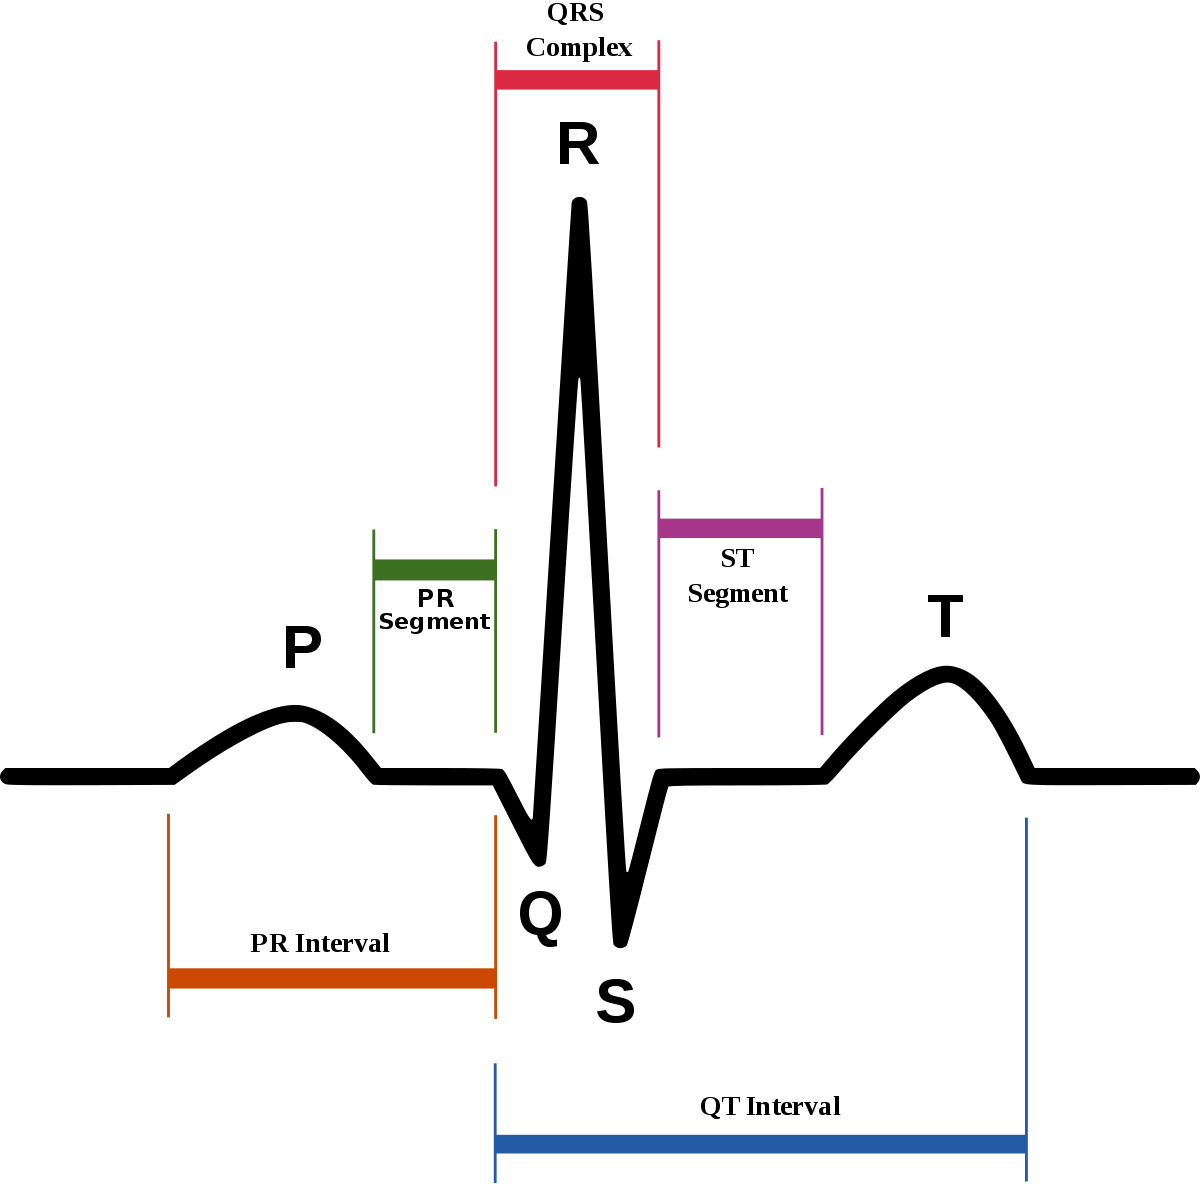
\includegraphics[width=0.6\textwidth]{Billeder/pqrst.png}
   \caption{EKG signal} 
   \label{fig:pqrst}
\end{figure}

\textbf{P bølge} repræsenterer depolarisering af atrierne. Impulser spredes fra sinusknude mod AV-knude og fra højre til venstre atrium. Kontraktion af atrierne forekommer 25 msek efter starten af p bølgen.

\textbf{PR interval} måles fra starten af p bølgen og til starten af QRS komplekset. Dette interval repræsenter den tid det tager for den elektriske impuls at rejse fra sinusknude til AV-knude.

\textbf{PR segment} er den flade linje mellem slutningen af p-bølgen og starten af QRS komplekset. Denne reflekterer den tids forsinkelse af AV-knude som forekommer således at ventriklerne kan fyldes.  

\textbf{QRS komplekset} repræsenterer den hurtige depolarisering af ventriklerne. Det elektriske signal er meget stærk, da ventriklernes muskler er meget mere massiv ift atrierne. 

\textbf{ST segment} forbinder QRS kompleks med t bølge. Repræsenter den tid det tager for ventriklerne at depolarisere.

\textbf{T bølge} repræsenter repolarisering af ventriklerne. Repolarisering af artierne ses ikke i EKG'et, da det finder sted mens ventriklerne depolariserer og QRS komplekset forekommer. 

\subsection{Pre- og afterload}

\textbf{Slagvolumen} er den mængde blod, som pumpes ud fra hjertet under hvert pulsslag, hos mennesket ca. 80 ml.

\textbf{Minutvolumen/cardiac output} er den mængde blod, hjertet pumper ud pr. minut; udregnes som produktet af hjertets slagvolumen og slagfrekvensen, dvs. pulsen. Hjertets minutvolumen er hos voksne personer i hvile ca. 5 l/min. 

Preload og afterload er to afgørende faktorer for, hvor meget blod hjertet pumper i et minut (minutvolumen).

\textbf{Preload} defineres som den mængde af blod som kommer ind i ventriklerne lige før hjertet kontraherer (systole). Mere blod giver mere udstrækning af ventriklerne, hvilket giver en øget preload. Jo større preload, jo kraftigere kontraktion og jo større slagvolumen. 

\textbf{Afterload} defineres som den mængde af modstand/tryk som ventriklen skal overkomme for at blodet kan bevæge over i aorta under systole. Hvis afterload øges (eksempelvis pga. hypertension) så vil den isovolumetriske kontraktionsfase forlænges fordi ventriklerne har brug for at generere et højere tryk og slagvolumen nedsættes. 

